\documentclass[12pt]{article}

\usepackage[margin=1in]{geometry}
\usepackage{multicol}
\usepackage{bookmark}
\usepackage{adjustbox}
\usepackage{mathtools}
\usepackage{amsmath}
\usepackage{amssymb}
\usepackage{amsthm}
\usepackage{amsfonts}
\usepackage{algorithmic}

\usepackage{pgfplots}
\pgfplotsset{compat=1.16}
\usepackage{tikz}
\usetikzlibrary{cd, arrows, decorations.markings}
\usepackage{graphicx}
\usepackage{rotating}
\usepackage{pst-solides3d}
\usepackage{xcolor}
\usepackage{hyperref}
\usepackage[cache=false]{minted}

\usepackage{fancyhdr}
\usepackage{tocloft}
\usepackage{caption}
\usepackage{soul}
\usepackage{cite}
\usepackage{textcomp}

\usepackage{wasysym}

% Sets and related operators
\newcommand{\nats}{\mathbb{N}}                            % Natural numbers
\newcommand{\pnats}{\mathbb{N}^+}                         % Positive natural numbers (excluding 0)

\newcommand{\ints}{\mathbb{Z}}                            % Integers
\newcommand{\pints}{\mathbb{Z}^+}                         % Positive integers
\newcommand{\nints}{\mathbb{Z}^-}                         % Negative integers

\newcommand{\rats}{\mathbb{Q}}                            % Rational numbers
\newcommand{\prats}{\mathbb{Q}^+}                         % Positive rational numbers
\newcommand{\nrats}{\mathbb{Q}^-}                         % Negative rational numbers

\newcommand{\reals}{\mathbb{R}}                           % Real numbers
\newcommand{\preals}{\mathbb{R}^+}                        % Positive real numbers
\newcommand{\nreals}{\mathbb{R}^-}                        % Negative real numbers

\newcommand{\irrats}{\mathbb{I}}                          % Irrational numbers

\newcommand{\pset}{\mathcal{P}}                           % Powerset
\newcommand{\card}{\abs}                                  % Cardinality
\newcommand{\topology}{\mathcal{T}}                       % Topology
\newcommand{\basis}{\mathcal{B}}                          % Basis
\newcommand{\oldemptyset}{\emptyset}                      % Old empty set
\renewcommand{\emptyset}{\varnothing}                     % New and nice empty set

% Operators
\DeclarePairedDelimiter\abs{\lvert}{\rvert}               % Absolute value
\DeclarePairedDelimiter\ceil{\lceil}{\rceil}              % Ceiling
\DeclarePairedDelimiter\floor{\lfloor}{\rfloor}           % Floor

% Other
\newcommand{\rarr}{\rightarrow}                           % Leftarrow
\newcommand{\larr}{\leftarrow}                            % Rightarrow (equivalent to \to)
\newcommand\und[1]{\underline{\smash{#1}}}                % Nice-looking underline
\renewcommand{\headrulewidth}{0.5pt}                      % Header rule width
\renewcommand{\footrulewidth}{0pt}                        % Footer rule width
\renewcommand{\baselinestretch}{1.5}                      % Make the line spacing equal to 1.5
\renewcommand{\cftsecleader}{\cftdotfill{\cftdotsep}}     % Add dots to the sections in the table of contents
\renewcommand{\contentsname}{\textbf{TABLE OF CONTENTS}}  % Change the name from "Contents" to the "Table of Contents"
\renewcommand{\cfttoctitlefont}{\hspace*{\fill}\Large}    % Filling the space for centering the table of contents' title
\renewcommand{\cftaftertoctitle}{\hspace*{\fill}}         % Filling the space for centering the table of contents' title

% Setting stuff
\setlength{\parindent}{0pt}                               % Remove indentations from paragraphs
\frenchspacing                                            % Sometimes latex creates unnecessarily large spaces after dots, this helps to avoid it (puts single spaces at the end of sentences)
\pagestyle{fancy}                                         % This allows to do fancy headers and footers
\fancyhf{}                                                % No additional page numbering (or other stuff such as references)
\cfoot{\thepage}                                          % Display page number at the bottom in the center
\hypersetup{                                              % Nice-looking urls
    colorlinks,
    linkcolor={blue!50!black},
    citecolor={blue!50!black},
    urlcolor={blue!50!black}
}

\rhead{\footnotesize{\MakeUppercase{The Topology of Robotic Configuration and Motion Planning}}}

% Definition environment
\theoremstyle{definition}
\newtheorem*{definition}{Definition}


% Title
\title{\textbf{The Topology of Robotic Configuration and Motion Planning}\\
{\small \textsuperscript{*}The paper is written in scope of the independent study course with Dr. Eric Westlund.}}

% Author
\author{David Oniani\\Luther College\\\href{mailto:oniada01@luther.edu}{oniada01@luther.edu}}

% Date
\date{January 30, 2019}


\begin{document}
\maketitle

%%%%%%%%%%%%%%%%%%%%%%%%%%%%%%%%%%%%%%%%%%%%%%%%%%%%%%%%%%%%%%%%%%%%%%%%%%%%%%%%%%%%%%%%%%%%%%%%%%%%

\begin{abstract}
\addcontentsline{toc}{section}{Abstract}

\noindent This paper explores the topological approach to the problem
of robot motion planning. Particularly, we will discuss the safe way
to coordinate automated guided vehicles or AGVs. AGVs are mobile robots
which are used extensively in manufacturing facilities. Since these robots
are costly and cannot tolerate collisions, one of the biggest challenges
in designing such facility is setting up mobile robot routes to achieve
the safe and efficient coordination of robots. The tools and concepts of
topology are naturally employed in this planning process. This paper
follows the bottom-up approach by first introducing concepts and then
building upon these ideas. It does not assume any background neither in
topology nor in robotics and is therefore accessible to most undergraduate
mathematics students with the knowledge of set theory.
\end{abstract}

%%%%%%%%%%%%%%%%%%%%%%%%%%%%%%%%%%%%%%%%%%%%%%%%%%%%%%%%%%%%%%%%%%%%%%%%%%%%%%%%%%%%%%%%%%%%%%%%%%%%

\newpage
\tableofcontents
\newpage

%%%%%%%%%%%%%%%%%%%%%%%%%%%%%%%%%%%%%%%%%%%%%%%%%%%%%%%%%%%%%%%%%%%%%%%%%%%%%%%%%%%%%%%%%%%%%%%%%%%%

\section*{\centering Configuration Spaces}
\addcontentsline{toc}{section}{Configuration Spaces}

We shall start by introducing the notion of configuration spaces.
The idea of configuration spaces comes from physics. In classical
mechanics, the configuration space is the vector space defined by
the generalized coordinates (coordinates that describe the configuration
of the physical system). Put it simply, the configuration space is
the set of all possible states that could exist in the physical system.
For instance, the configuration space of some particle in the room is
the set of all points/states of the type $(x, y, z)$ where $x, y$ and $z$
are the coordinates bounded by the room. If the room is a $3 \times 3 \times 3$
cube then we define the configuration space of the particle by
$$C^3(\text{room}) = \{(x, y, z) \mid 0 \leq x, y, z \leq 3\}.$$
In other words, the configuration space of the particle, is all of
$3 \times 3 \times 3$ cube (this example obviously assumes that the
particle is allowed to move freely in the room). The configuration space
of the same particle in a spherical room, however, would be the set of all
points that are in a sphere.

\bigskip

It appears that the physical notion of configuration spaces is very much
connected to that of mathematics. In fact, the idea is the same but rather
generalized. To better understand configuration spaces, let us first go
through several \textit{classic} examples.

\bigskip

\cite{1} Consider a planar system where we have a rod with a fixed end that can rotate freely. Then it is
easy to see that the space of all possible configurations of the rotating rod is a circle.

\begin{figure}[H]
\centering
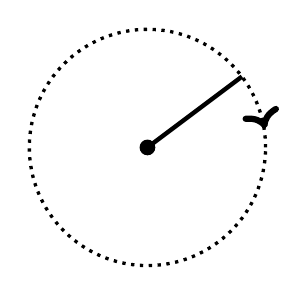
\begin{tikzpicture}
    % Circle
    \draw[
        black,
        very thick,
        dotted,
        decoration={markings, mark=at position 0.05 with {\arrow[draw=black, line width=2.25pt]{<}}},
        postaction={decorate}
        ]
        (2, 2) circle (1.5);

    % Rotating rod
    \draw[black, ultra thick] (2, 2) -- (3.2, 2.9);

    % Fixed endpoint
    \fill (2, 2) circle (0.1);
\end{tikzpicture}
\caption*{Circle obtained by the rotational motion of the rod.}
\end{figure}

In other words, as the rod rotates, it creates the circle around itself
with the radius equal to the length of the rod. This configuration space
is also known as $S^1$.

\bigskip

\cite{2} On the other hand, the configuration space of the two-rod
system in 3D space where one rod is fixed and the other one is attached to it (also known as a 2R robot)
is a torus. This space is also known as $S^1 \times S^1$ configuration space.

\begin{figure}[H]
\centering
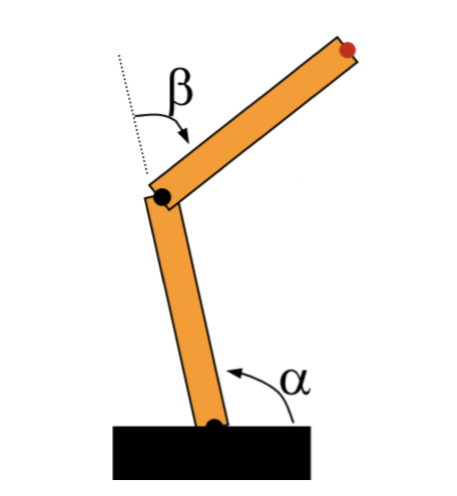
\includegraphics[width=4cm, height=4cm]{two-rod-system}
\caption*{A two-rod system ($2R$ robot).}
\end{figure}

We already know that a rod with fixed end generates a circle. In this case,
we have two rods: one attached to the ground and the other one attached to the end
of the first one. Then obviously both of the rods can go through a full circle
of states and therefore, create a configuration space which geometrically represents a torus.

\begin{figure}[H]
    \centering
    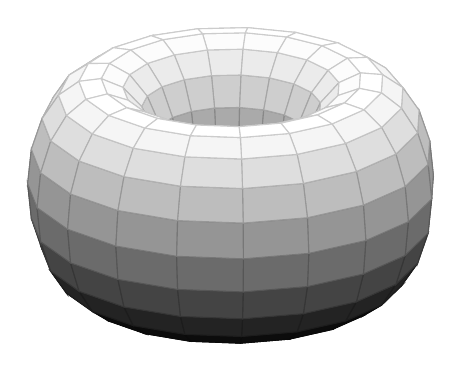
\begin{tikzpicture}
        \begin{axis}[hide axis]
           \addplot3[
               surf,
               colormap/blackwhite,
               samples=20,
               domain=0:2*pi,
               y domain=0:2*pi,
               z buffer=sort
             ]
             ( {(2 + cos(deg(x))) * cos(deg(y + pi/2))}, 
               {(2 + cos(deg(x))) * sin(deg(y + pi/2))}, 
               {sin(deg(x))}
             );
        \end{axis}
      \end{tikzpicture}
    \caption*{A torus obtained by the motion of two-rod system.}
\end{figure}

As of now, this is all we need to know about the configuration spaces.
This idea will be very useful once we learn more about other topological concepts.

%%%%%%%%%%%%%%%%%%%%%%%%%%%%%%%%%%%%%%%%%%%%%%%%%%%%%%%%%%%%%%%%%%%%%%%%%%%%%%%%%%%%%%%%%%%%%%%%%%%%

\section*{\centering Topological Spaces}
\addcontentsline{toc}{section}{Topological Spaces}

The fundamental idea in topology is that of a topological space.
We will use this idea to then introduce and define other important concepts.

\begin{definition}
\cite{3} A \textit{\textbf{topology}} on a set $X$ is a collection $\topology$ of subsets of $X$ having
the following properties:

\begin{itemize}
\item[(1)]
$\emptyset$ and $X$ are in $\topology$.

\item[(2)]
The union of the elements of any subcollection of $\topology$ is in $\topology$.

\item[(3)]
The intersection of the elements of any finite subcollection of $\topology$ is in $\topology$.
\end{itemize}

A set $X$ for which a topology $\topology$ has been specified is called a \textit{\textbf{topological space}}.
\end{definition}

Let us first look at some examples. Consider a set $X = \{a, b, c\}$.
Then we can define a topology on $X$ by $\topology = \{\emptyset, \{a, b, c\}, \{a, b\}, \{c\}\}$.
Observe that $\emptyset, X \in \topology$ therefore the first criterion is satisfied.
It is easy to see that arbitrary unions will be in $\topology$ since the only ``interesting''
case is when we consider $\{a, b\}$ and $\{c\}$, but in this case $\{a, b\} \cup \{c\} = \{a, b, c\} \in \topology$.
This satisfies the second requirement. Finally, any arbitrary intersection of the finite subcollections of $\topology$
is also in $\topology$ and therefore, we conclude that $\topology$ is indeed a topology on $X$.
Hence, $X$ is a topological space (note that, properly speaking, a topological space is an ordered pair $(X, \topology)$,
but we often omit mentioning $\topology$ and say that $X$ is a topological space).

\bigskip

At this point, you might have already noticed that one could always define more than one topology
for a given set. In the previous example, sets $\pset{(x)}$ (powerset of $x$) and $\{\emptyset, X\}$
are also topologies on $X$ called \textit{discrete} and \textit{indiscrete} topologies. In fact, for any set $X$,
$\pset{(x)}$ and $\{\emptyset, X\}$ will always be two distinct topologies on $X$.

\bigskip

We will now get acquainted with the notion of the \textit{open set}.

\begin{definition}
\cite{4}  If $X$ is a topological space with topology $\topology$, we say that a subset $U$ of $X$ is an
\textbf{open set} of $X$ if $U$ belongs to the collection $\topology$.
\end{definition}

Consider our topology $\topology = \{\emptyset, \{a, b, c\}, \{a, b\}, \{c\}\}$ on the topological space $X = \{a, b, c\}$.
Then notice that $\emptyset, \{a, b, c\}, \{a, b\}, \{c\} \in \topology$ and therefore, all are open sets.

%%%%%%%%%%%%%%%%%%%%%%%%%%%%%%%%%%%%%%%%%%%%%%%%%%%%%%%%%%%%%%%%%%%%%%%%%%%%%%%%%%%%%%%%%%%%%%%%%%%%

\section*{\centering Continuous Functions and Homeomorphisms}
\addcontentsline{toc}{section}{Continuous Functions and Homeomorphisms}

The notion of continuous functions is familiar to most high-school students.
Most people associate them with a nice-looking monotonically increasing or decreasing
functions with no leaps or jumps. There are several definitions for a function continuity.
Here is the calculus definition.

\begin{definition}
\cite{5} A function $f(x)$ is continuous at a point $x = c$ if and only if it meets the following
three conditions:\\
1. $f(c)$ exists ($c$ lies in the domain of $f$).\\
2. $\lim_{x \to c}f(x)$ exists ($f$ has a limit as $x \to c$).\\
3. $\lim_{x \to c}f(x) = f(c)$ (the limit equals to the function value).
\end{definition}

In topology we cannot use this definition since the definition assumes
that one could take a limit of the function. This, however, is sometimes very difficult or nearly impossible
when considering functions defined over more abstract sets such as the configuration space
of AGV. Now, we shall introduce more general notion of continuity.

\begin{definition}
\cite{6} Let $X$ and $Y$ be topological spaces. A function $f : X \to Y$ is said to be \textbf{continuous} if
for each open subset $V$ of $Y$, the set $f^{-1}(V)$ is an open subset of $X$.
\end{definition}

It is important to note that in this definition $f^{-1}(V)$ does not refer to the inverse of the function.
Therefore, we are not assuming that $f : X \rarr Y$ is a bijection. $f^{-1}(V)$ refers to the preimage
(the elements of the domain that map to some elements in the codomain) of the function. In other words,
the function $f : X \to Y$ over two topological spaces $X$ and $Y$ is continuous if and only if every open
set in the image is mapped by an open set from the preimage.

\bigskip

This is the case where the visualization might be useful to see how the definition of continuous functions really works.
Consider a continuous function $f : X \to Y$ where $X$ and $Y$ are topological spaces with topologies $\topology_X$ and $\topology_Y$.

\begin{figure}[H]
    \centering
    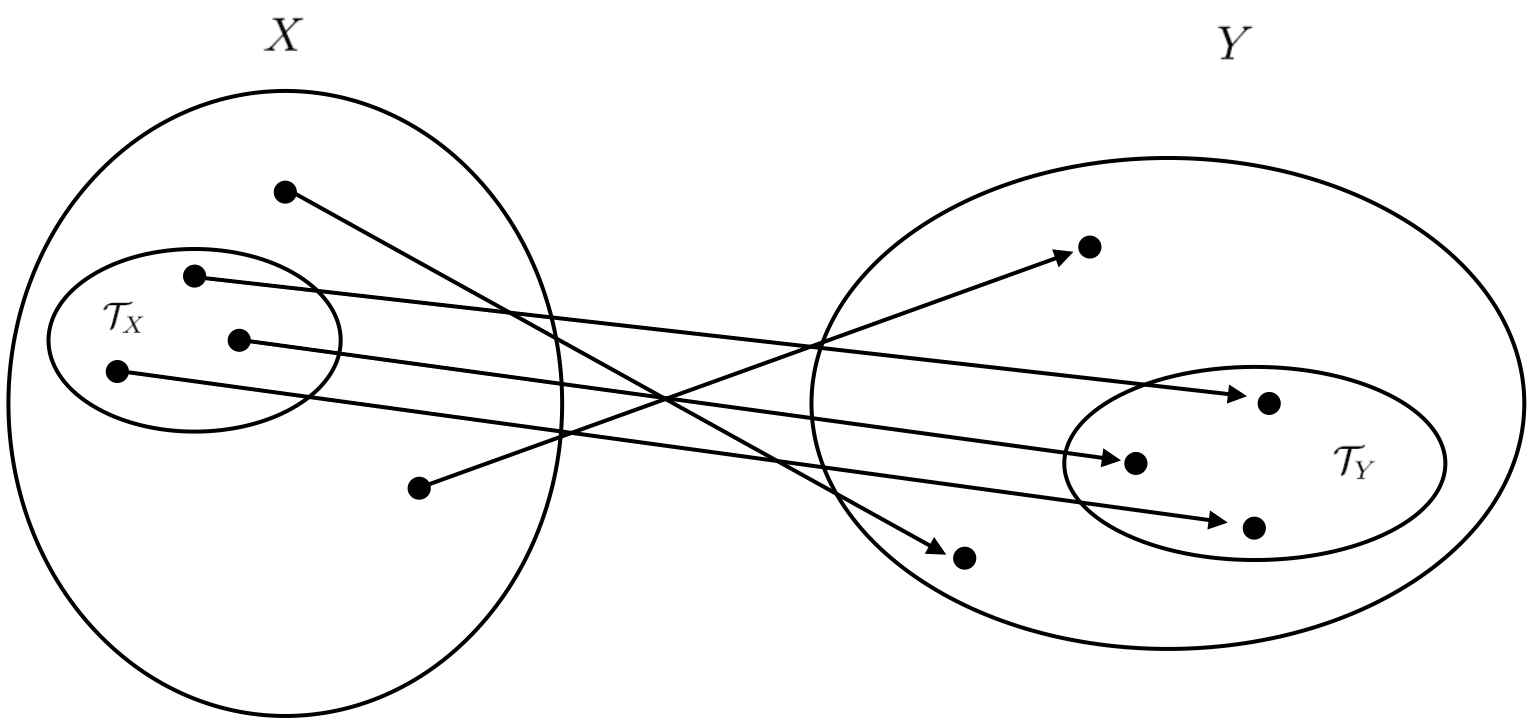
\includegraphics[width=7.5cm, height=4.5cm]{continuous-function}
    \caption*{A continuous function $f : X \to Y$.}
\end{figure}

In the figure above, the big blobs $X$ and $Y$ are topological spaces and the smaller blobs $\topology_X$
and $\topology_Y$ are the topologies on $X$ and $Y$ correspondingly. By the definition, the elements in $\topology_X$
or $\topology_Y$ are open sets. Then notice that the function $f : X \to Y$ shown above is continuous. All the points
which are in $\topology_Y$ have a preimage in $\topology_X$. Note that there are points in $Y$ that do not have a preimage
in $\topology_X$, but it is of no importance to the continuity of $f$ since it must be open sets in $Y$ (not just any set)
that must have an open preimage.

\bigskip

The function below, however, is not continuous as there is one point that is not in $\topology_X$
but maps to a point in $\topology_Y$ (it is highlighted with the red arrow).

\begin{figure}[H]
    \centering
    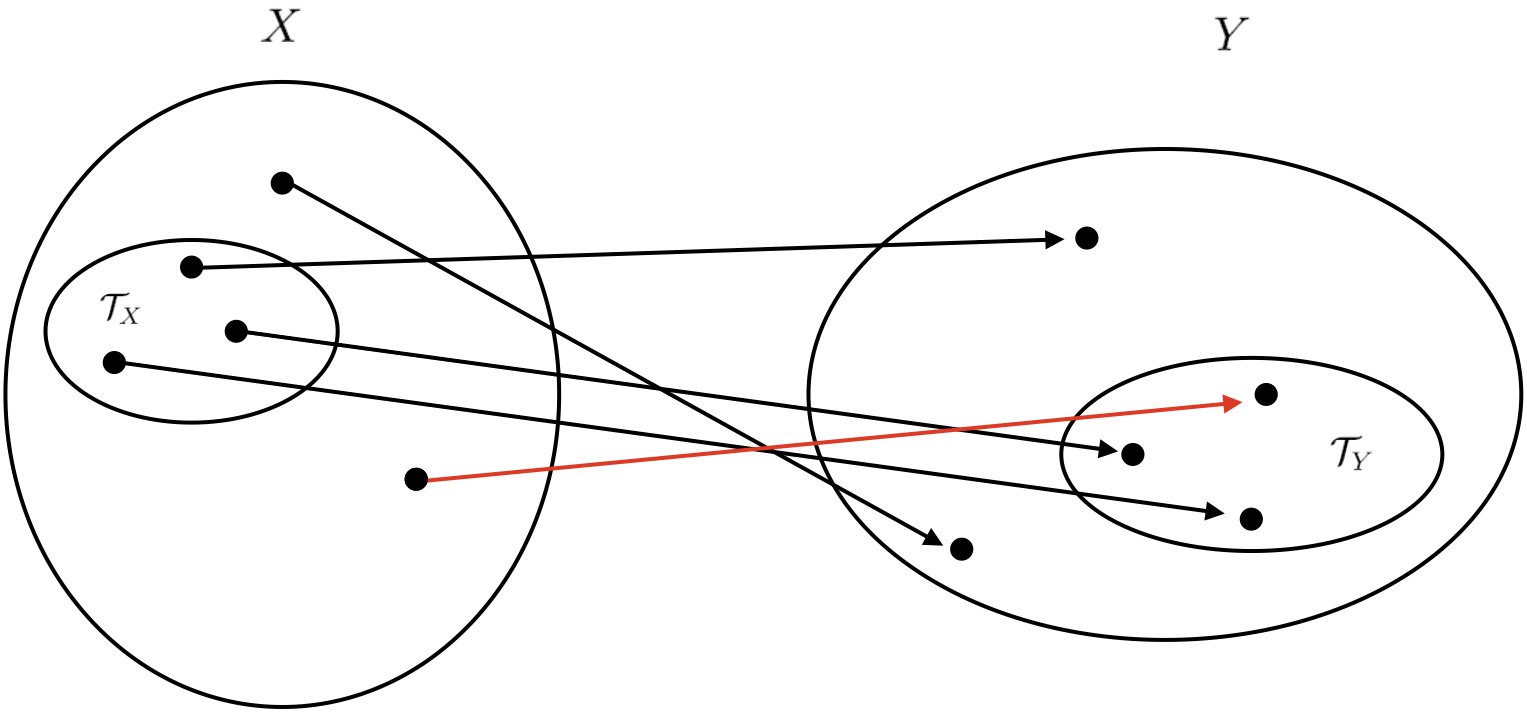
\includegraphics[width=7.5cm, height=4.5cm]{discontinuous-function}
    \caption*{A discontinuous function $f : X \to Y$.}
\end{figure}

\bigskip

Now that we are familiar with the notion of continuous functions, we shall introduce a new concept, that of homeomorphism.

\begin{definition}
\cite{7} Let $X$ and $Y$ be topological spaces; let $f : X \to Y$ be a bijection. If both the function $f$
and the inverse function
$$f^{-1} : Y \to X$$
are continuous, then $f$ is called a homeomorphism.
\end{definition}

The important fact about homeomorphisms is that they preserve the \textit{topological structure}.
Roughly speaking, a topological space is a geometric object. We say that two objects are homeomorphic
if one can be obtained from the other by continuous deformation (vice versa). From the topological viewpoint,
homeomorphism implies equality and therefore, two objects are considered the same if they are homeomorphic
to each other.

%%%%%%%%%%%%%%%%%%%%%%%%%%%%%%%%%%%%%%%%%%%%%%%%%%%%%%%%%%%%%%%%%%%%%%%%%%%%%%%%%%%%%%%%%%%%%%%%%%%%

\section*{\centering Connectedness and Path Connectedness}
\addcontentsline{toc}{section}{Connectedness and Path Connectedness}

One of the important ideas in topology is that of connectedness.
This idea is used extensively in various other fields of mathematics such as graph theory and knot theory.
Let us first define connectedness.

\begin{definition}
\cite{8} Let $X$ be a topological space. A \textbf{separation} of $X$ is a pair $U, V$ of disjoint
nonempty open subsets of $X$ whose union is $X$. The space $X$ is said to be \textbf{connected}
if there does not exist a separation of $X$.
\end{definition}

Consider a topological space $X = \{a, b, c\}$ with a topology $\topology = \{\emptyset, \{a, b, c\}, \{a, b\}, \{c\}\}$.
Then it is easy to see that $X$ is a disconnected space. Sets $\{a, b\}$ and $\{c\}$ are open since $\{a, b\}, \{c\} \in \topology$.
Besides, $\{a, b\} \cap \{c\} = \emptyset$ and $\{a, b\} \cup \{c\} = \{a, b, c\} = X$ with $\{a, b\}, \{c\} \neq \emptyset$.
Hence, $U = \{a, b\}$ and $V = \{c\}$ is a pair of disjoint open subsets of $X$ whose union is $X$
and therefore $U, V$ is a separation of $X$. This means that $X$ is a disconnected space.

\bigskip

On the other hand, a topological space $Y = \{a, b\}$ with a topology $\topology = \{\emptyset, \{a, b\}, \{a\}\}$
is a connected space as there is no pair of disjoint nonempty open subsets of $Y$ such that their union is $Y$.
In other words $Y$ has no separation. Note that $\emptyset \cup \{a, b\} = \{a, b\} = Y$, but it must be \und{nonempty}
sets whose union is $Y$. Therefore, $\emptyset, \{a, b\}$ is not a separation of $Y$.

\bigskip

Knowing what it means for a topological space to be connected, we can now introduce the notion
of path connectedness.

\begin{definition}
\cite{9} Given points $x$ and $y$ of the space $X$, a \textbf{path} in $X$ from $x$ to $y$ is a 
continuous map $f : [a, b] \to X$ of some closed interval in the real line into $X$, such
that $f(a) = x$ and $f(b) = y$. A space $X$ is said to be \textit{\textbf{path connected}} if every pair of
points of $X$ can be joined by a path in $X$.
\end{definition}

Path connected spaces are certainly related to the connected spaces.
\cite{10} In fact, one could easily verify that path connectedness implies connectedness.
Therefore, every path-connected space is connected.

\bigskip

There is an important theorem on path connected spaces which implies that a product of two path connected spaces is path connected.
Let us prove this theorem.

\begin{proof}
Suppose that $X$ and $Y$ are path-connected spaces.
Let $x_1 \times x_2, y_1 \times y_2 \in X \times Y$.
Notice that $X \times y_1$ is homeomorphic to $X$
and thus, is path-connected. Therefore, there exists
a continuous function $f : [0, 1] \to X \times y_1$
with $f(0) = x_1 \times y_1$ and $f(1) = x_2 \times y_2$.
Besides, $x_2 \times Y$ is homeomorphic to $Y$ and thus,
is path-connected. Therefore, there exists a continuous
function $g$ such that $g : [0, 1] \to x_2 \times Y$
with $g(0) = x_2 \times y_1$ and $g(1) = x_2 \times y_2$.
Let's now define a function $h$ in the following way:
$$
h(x) = 
\begin{cases}
f(\frac{x}{2}) \mbox{ if } 0 \leq x \leq \frac{1}{2}\\
f(\frac{x}{2} + \frac{1}{2}) \mbox{ if } \frac{1}{2} < x \leq 1.
\end{cases}
$$
The according to the \cite{11} \textbf{the pasting lemma},
$h$ is continuous. Besides, $h(0) = f(\frac{0}{2}) = f(0) = x_1 \times y_1$
and $h(1) = g(\frac{1}{2} + \frac{1}{2}) = g(1) = x_2 \times y_2$.
Therefore, $h$ is a path from $x_1 \times y_1$ to $x_2 \times y_2$
and because $x_1 \times y_1$ and $x_2 \times y_2$ are arbitrary, we have that
$X \times Y$ is path-connected.
\end{proof}

Now, because the product of two spaces is path connected, we can generalize this
notion to $n$ path connected spaces $X_1, X_2, \dots, X_N$ and say that the product
$X_1 \times X_2 \times \dots \times X_N$ is also path connected. The proof of this
using induction is almost trivial so we will not go through it in this paper.

%%%%%%%%%%%%%%%%%%%%%%%%%%%%%%%%%%%%%%%%%%%%%%%%%%%%%%%%%%%%%%%%%%%%%%%%%%%%%%%%%%%%%%%%%%%%%%%%%%%%

\section*{\centering Configuration Spaces Revisited - Robotic Configurations}
\addcontentsline{toc}{section}{Configuration Spaces Revisited - Robotic Configurations}

In previous sections, we went through what is called a configuration space.
Yet, we did not have a precise definition for it since it varies from field to field.
Let us now define what a configuration space means in the robotics context.

\begin{definition}
\cite{12} A \textit{\textbf{configuration}} of a robot is a specification of the position of all points of a robot.
The \textit{\textbf{configuration space}} of a robot is the space of all configurations of a robot.
\end{definition}

Suppose that we have a robot $R$ that can move freely on a line $L$. Then we can model the robot as
a point with a coordinate $x_R$. The configuration space for this robot is

$$C^1(L) = \{x_R \mid x_R \in L\} = L = L^1.$$

with every point in the room being a unique configuration of the robot.

\bigskip

What if we had 2 robots (say $R_1$ and $R_2$) that can move freely?
Then the configuration space would be $C^2$ which can be represented as the set
$$C^2(L) = \{(x_{R_1}, x_{R_2}) \mid x_{R_1}, x_{R_2} \in L\} = L \times L = L^2.$$
The result here is somewhat natural. If we have one robot moving on a line, we have a configuration
space $L$. If there are two robots, the configuration changes from a single point to a 2-tuple
($(x_{R_1}, x_{R_2})$ in the case) which yields a configuration space equal to $L^2$.

\bigskip

In general, the configuration space for $n$ robots $R_1, R_2, \dots, R_n$ that can move freely on a line $L$ is

$$C^n(L) = \{(x_{R_1}, x_{R_2}, \dots, x_{R_n}) \mid x_{R_1}, x_{R_2}, \dots, x_{R_n} \in L\} = \underbrace{L \times L \times \dots \dots L}_{n \ \text{times}} = L^n.$$

In fact, we could generalize this notion even further. Instead of having
$n$ robots moving on a line $L$, consider $n$ robots moving on some $k$-dimensional space $L^k$.
Then each configuration will be a tuple consisting of $n$ number of $k$-tuples and the configuration
space of all $n$ robots will be a set of all such tuples. Therefore, we have
\begin{equation*}
    \begin{split}
    C^n(L^k) = \{((x_{R_{1, 1}}, x_{R_{1, 2}}, \dots, x_{R_{1, k}}), \dots, (x_{R_{n, 1}}, \dots, x_{R_{n, k}})) \mid \ & (x_{R_{1, 1}}, x_{R_{1, 2}}, \dots, x_{R_{1, k}}),\\
    &\dots,\\
    &(x_{R_{n, 1}}, \dots, x_{R_{n, k}}) \in L^K\}\\
    &= \underbrace{L^k \times L^k \times \dots \times L^k}_{n \ \text{times}}\\
    &= L^{nk}.
    \end{split}
\end{equation*}

where $(x_{R_{1, 1}}, x_{R_{1, 1}}, \dots, x_{R_{1, k}})$ is the coordinate of $R_1$, $(x_{R_{2, 1}}, x_{R_{2, 1}}, \dots, x_{R_{2, k}})$ is the coordinate of $R_2$, etc.

%%%%%%%%%%%%%%%%%%%%%%%%%%%%%%%%%%%%%%%%%%%%%%%%%%%%%%%%%%%%%%%%%%%%%%%%%%%%%%%%%%%%%%%%%%%%%%%%%%%%

\section*{\centering Safe Robotic Configurations}
\addcontentsline{toc}{section}{Safe Robotic Configurations}

At this point, we have enough machinery to understand safe robotic configurations.
Let us model each robot with a point that moves through a topological space representing
the robot routes in the factory.

\bigskip

Consider two robots $R_1$ and $R_2$ moving through the line represented by $L$ ($L$ is obviously a topological space).
Then the configuration space for these robots is
$$C = \{(x_{R_1}, x_{R_2}\} \mid x_{R_1}, x_{R_2} \in L\} = L \times L = L^2.$$

\bigskip

Now, since $x_{R_1}$ and $x_{R_2}$ represent the coordinates of the robots, we cannot allow them to be the same.
In other words, if $x_{R_1} = x_{R_2}$, we have a collision. We therefore modify our configuration space $C$
to eliminate all the configurations where $x_{R_1} = x_{R_2}$. Let us call this new configuration space $SC$
(a safe configuration space) with
$$SC = \{(x_{R_1}, x_{R_2}) \mid x_{R_1}, x_{R_2} \in \reals, x_{R_1} \neq x_{R_2}\}.$$

\bigskip

It is really helpful to think about this configuration space geometrically.
Particularly, let's think about this space as a small chunk of the $XOY$ coordinate system.
To do this, we will need to do some transformations. Since $L$ is a line we might as well
represent it as a closed interval $L = [0, l]$ where $l$ is the length of the line $L$ and therefore
$l \in \reals$. Now we can say that both robots $R_1$ and $R_2$ are moving through the interval $[0, l]$.
Let us now consider the motion of $R_1$ and $R_2$ independently. To do this, we make a copy
of the interval $[0, l]$, put one interval as an $X$ axis and the other one as the $Y$ axis.

\begin{figure}[H]
    \centering
    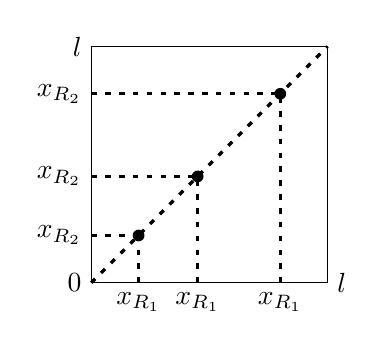
\begin{tikzpicture}[scale=1.5]
        % Square
        \draw (0, 0) -- (2, 0) -- (2, 2) -- (0, 2) -- (0, 0);
        % Diagonal
        \draw [very thick, dash pattern=on 2pt off 3pt] (0, 0) -- (2, 2);
        % Points
        \node [left] at (0, 2) {$l$};
        \node [right] at (2, 0) {$l$};
        \node [left] at (0, 0) {$0$};
        % 0.4, 0.4
        \node [below] at (0.4, 0) {$x_{R_1}$};
        \node [left] at (0, 0.4) {$x_{R_2}$};
        \node at (0.4, 0.4) [circle, fill, inner sep=1.5pt]{};
        % 0.9, 0.9
        \node [below] at (0.9, 0) {$x_{R_1}$};
        \node [left] at (0, 0.9) {$x_{R_2}$};
        \node at (0.9, 0.9) [circle, fill, inner sep=1.5pt]{};
        % 1.6, 1.6
        \node [below] at (1.6, 0) {$x_{R_1}$};
        \node [left] at (0, 1.6) {$x_{R_2}$};
        \node at (1.6, 1.6) [circle, fill, inner sep=1.5pt]{};
        % 0.4, 0.4
        \draw [very thick, dash pattern=on 2pt off 3pt] (0, 0.4) -- (0.4, 0.4);
        \draw [very thick, dash pattern=on 2pt off 3pt] (0.4, 0) -- (0.4, 0.4);
        % 0.9, 0.9
        \draw [very thick, dash pattern=on 2pt off 3pt] (0, 0.9) -- (0.9, 0.9);
        \draw [very thick, dash pattern=on 2pt off 3pt] (0.9, 0) -- (0.9, 0.9);
        % 1.6, 1.6
        \draw [very thick, dash pattern=on 2pt off 3pt] (0, 1.6) -- (1.6, 1.6);
        \draw [very thick, dash pattern=on 2pt off 3pt] (1.6, 0) -- (1.6, 1.6);
    \end{tikzpicture}
    \caption*{The configuration space $C$ as a chunk of $XOY$ coordinate system.}
\end{figure}

From the picture above, it is easy to see that the points where $x_{R_1} = x_{R_2}$
are the points on the \textbf{diagonal} of the square bounded by interval $[0, l]$ on $X$ axis
and its copy on the $Y$ axis. We denote this diagonal by $\Delta$. Then we can simply
say that

$$SC = C - \Delta.$$

In the general case with $n$ robots and the topological space $X$, it is easy to see that
$$SC^n = \underbrace{X \times X \times \dots \times X}_{n \ \text{times}} - \Delta \ \text{where} \ \Delta = \{(x_{R_1}, x_{R_2}, \dots, x_{R_n}) \mid x_{R_i} = x_{R_j} \ \text{for some} \ i \neq j\}.$$

We are basically taking the product of $n$ copies of $X$ because we have $n$ robots
and account for the position of each robot independently. Every configuration in this
configuration space will look like $(x_{R_1}, x_{R_2}, \dots x_{R_n})$ and we eliminate each
configuration for which there exists $x_{R_i}$ and $x_{R_j}$ such that $x_{R_i} = x_{R_j}$ with $i \neq j$.
This means that we do not allow any two robots to have the same coordinates in any configuration which
ensures that there are no collisions.

%%%%%%%%%%%%%%%%%%%%%%%%%%%%%%%%%%%%%%%%%%%%%%%%%%%%%%%%%%%%%%%%%%%%%%%%%%%%%%%%%%%%%%%%%%%%%%%%%%%%

\section*{\centering Safe Robotic Relocations}
\addcontentsline{toc}{section}{Safe Robotic Relocations}

Now that we know about safe robotic configurations, let us model the relocation
of $n$ robots in the space $X$. To do this, we need to use a path in $SC^n(X)$.
Suppose that initially the robots had the configuration $(I_1, I_2, \dots, I_n)$
where $I_j$ is the initial position of the $j$-th robot. Then we define what is
called the \textbf{relocation} of these $n$ robots.

\begin{definition}
\cite{13} We define a \textit{\textbf{relocation}} of the $n$ robots from the initial configuration
$I = (I_1, \dots, I_n)$ to the finial configuration $F = (F_1, \dots, F_n)$ to be a path
$p : [0, 1] \to SC^n(X)$ such that $p(0) = I$ and $P(1) = F$.
\end{definition}

Since the robots are mapped to the configuration in $SC^n(X)$, by the definition of $SC$,
there is no way that any two robots will occupy the same coordinate and therefore, the map
will ensure that there are no collisions.

\bigskip

We can now introduce the notion of \textbf{attainability} of configurations using which we will define
some other important concept.

\begin{definition}
\cite{14} Given two configurations of the robots, $M = (M_1, \dots, M_n)$ and $N = (N_1, \dots, N_n)$,
we say that $N$ is \textit{\textbf{attainable}} from $M$ if there is a relocation of the robots
from $M$ to $N$.
\end{definition}

Now let's apply the definition of path connectedness that we covered a few chapter ago.
Notice that if the safe configuration space $SC^n(X)$ is path connected, then every configuration
is attainable from every other one and therefore, robots can move freely in the space.
In this case, we say that the robots are \textbf{freely transportable in} $X$.

\bigskip

The notion of free transportability is of the utmost important to robotics. We will spend the
rest of the paper exploring the free transportability under various robotic configurations.

%%%%%%%%%%%%%%%%%%%%%%%%%%%%%%%%%%%%%%%%%%%%%%%%%%%%%%%%%%%%%%%%%%%%%%%%%%%%%%%%%%%%%%%%%%%%%%%%%%%%

\section*{\centering Determining Free Transportability}
\addcontentsline{toc}{section}{Determining Free Transportability}

\subsection*{\centering Motion on Line $L$}
\addcontentsline{toc}{subsection}{Motion on Line $L$}

Consider two robots $R_1$ and $R_2$ on the line $L$ that we have discussed previously.
We know that the safe configuration space for two robots is the square without the diagonal.
Note that we consider the motion of $R_1$ robot on the horizontal line segment $[0, l]$
and the motion of $R_2$ robot on the vertical $[0, l]$ line segment.

\begin{figure}[H]
    \centering
    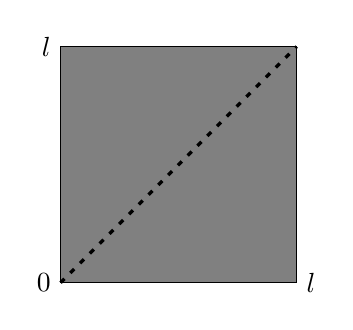
\begin{tikzpicture}[scale=1.5]
        % Draw the square
        \draw [fill=gray] (0, 0) -- (2, 0) -- (2, 2) -- (0, 2) -- (0, 0);
        % Points
        \node [left] at (0, 2) {$l$};
        \node [right] at (2, 0) {$l$};
        \node [left] at (0, 0) {$0$};
        % Lines
        \draw [very thick, dash pattern=on 2pt off 3pt] (0, 0) -- (2, 2);
    \end{tikzpicture}
    \caption*{A safe configuration space for two robots moving on the line $L$.}
\end{figure}

Then this safe configuration space is not path connected (recall that path connectedness
means that every pair of points of $SC$ can be joined by a path in $SC$). Observe that the safe configuration
space $SC$ is the union of two sets $U_1 = \{(x_{R_1}, x_{R_2} \mid x_{R_1}, x_{R_2} \in L, x_{R_1} < x_{R_2}\}$
and $U_2 = \{(x_{R_1}, x_{R_2} \mid x_{R_1}, x_{R_2} \in L, x_{R_2} < x_{R_1}\}$ where $U_1$ is the set in which $R_1$
is to the left of $R_2$ and $U_2$ is the set where $R_2$ is to the left of $R_1$. Notice that one of the sets has all
the configurations that lie above the excluded diagonal and the other one has all the configurations that lie below the
excluded diagonal. It is easy to show that this safe configuration space is not path connected. Take one point on the
one side of the diagonal and the other one on the other side (in other words, consider one configuration from the set
$U_1$ and the other one from the set $U_2$). If one would connect these points, there would not be a way to avoid
intersection of the diagonal.

\begin{figure}[H]
    \centering
    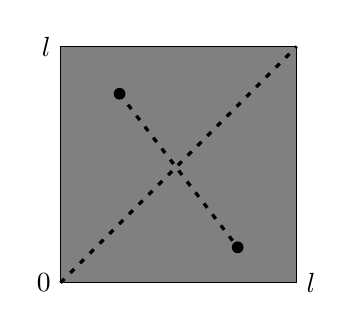
\begin{tikzpicture}[scale=1.5]
        % Draw the square
        \draw [fill=gray] (0, 0) -- (2, 0) -- (2, 2) -- (0, 2) -- (0, 0);
        % Points
        \node [left] at (0, 2) {$l$};
        \node [right] at (2, 0) {$l$};
        \node [left] at (0, 0) {$0$};
        \node at (0.5, 1.6) [circle, fill, inner sep=1.5pt]{};
        \node at (1.5, 0.3) [circle, fill, inner sep=1.5pt]{};
        % Lines
        \draw [very thick, dash pattern=on 2pt off 3pt] (0, 0) -- (2, 2);
        \draw [very thick, dash pattern=on 2pt off 3pt] (0.5, 1.6) -- (1.5, 0.3);
    \end{tikzpicture}
    \caption*{An attempt to connect two points from one side of the excluded diagonal to the other.}
\end{figure}

Thus, the safe configuration space $SC$ is not path connected and by the definition of
free transportability, $R_1$ and $R_2$ are not freely transportable in $L$.

\subsection*{\centering Motion on Circle $S^1$}
\addcontentsline{toc}{subsection}{Motion on Circle $S^1$}

Consider two robots $R_1$ and $R_2$ on the configuration space $S^1$ from the first section.
It is interesting to know what would the configuration space look like in this case.
We know that the configuration space $S^1$ is a circle. Then we consider the motion of $R_1$ and $R_2$ independently.
Let us now apply the same trick as we did with two robots on the line $L$. But now, since a circle is a 2D object,
we need to do it in the 3D space. Therefore, it is helpful to think about $XOYZ$ coordinate system.
We put a circle for $R_1$ on the $XOY$ plane and the circle for $R_2$ on the circle for $R_1$ circle in the way that
that these two circles share only one point. For simplicity, we will refer to these circles as $R_1$ and $R_2$
in all further correspondence. The picture below is the visualization of our approach.

\begin{figure}[H]
    \centering
    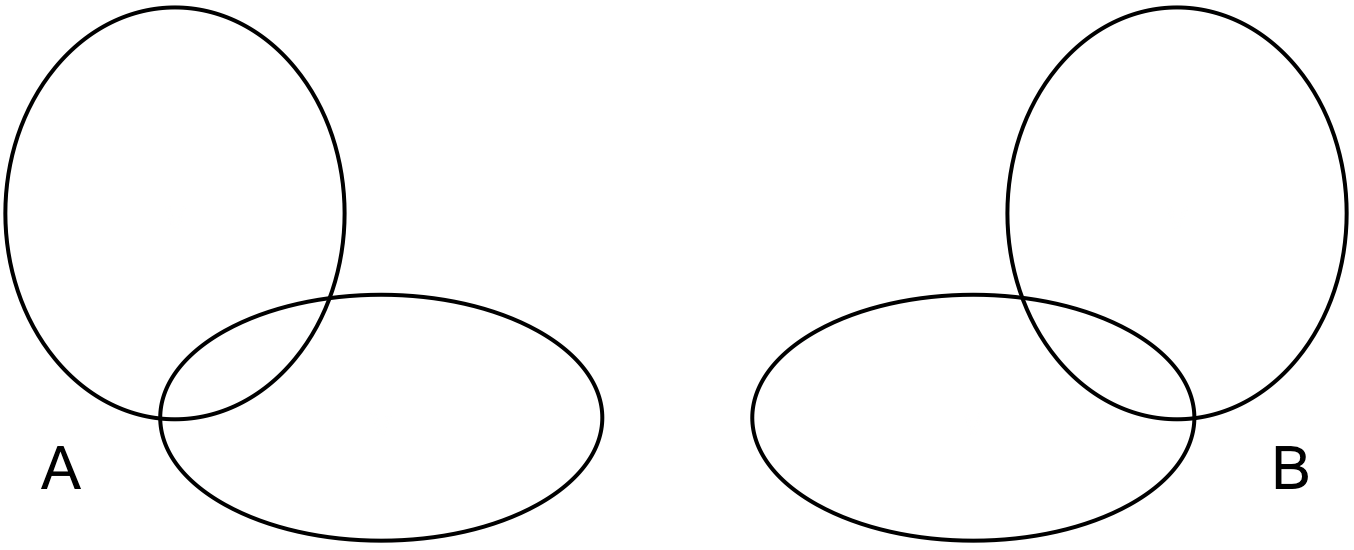
\includegraphics[width=10cm, height=5cm]{two-circles}
    \caption*{Figure A shows the first position of the circle and picture B the other one after sliding.}
\end{figure}

Recall that each configuration looks like $(x_{R_1}, x_{R_2})$.
Then to get all the configurations we keep the circle on the bottom (on the $XOY$ plane) fixed and slide the circle
on the $XOZ$ plane one point at a time. Each of these slides will generate a set of configurations which would be a set
of all points of upper circle paired with a single point on the bottom circle. We will continue this motion exhaustively,
until there are no points on the bottom circle. Figure B shows the picture when we are halfway through. Geometrically,
however, it is easy to see that the shape we get is a torus (\cite{15} in fact, the configuration space for $n$ robots on
the circle is the $n$-tori).

\bigskip

Obviously, we also want to know what is the safe configuration space for these two robots.
Here we will use another trick. Notice that we can glue the edges of a square to obtain a torus.
Therefore, we can ``unfold" the torus to get the square. We can represent the torus as a square
with opposite sides identified.

\begin{figure}[H]
    \centering
    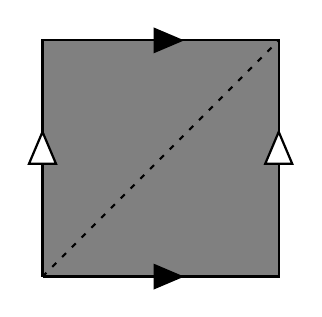
\begin{tikzpicture}[scale=1.5]
        \draw [thick, fill=gray] (0, 0) -- (2, 0) -- (2, 2) -- (0, 2) -- (0, 0);
        \draw [black, thick, dash pattern=on 2pt off 3pt] (0, 0) -- (2, 2);
        \tikzset{arrows={-Triangle[angle=45:12pt, black, fill=black]}}
        \draw [thick] (0, 0) -- (1.2, 0);
        \draw [thick] (0, 2) -- (1.2, 2);
        \tikzset{arrows={-Triangle[angle=45:14pt, black, fill=white]}}
        \draw [thick] (0, 0) -- (0, 1.25);
        \draw [thick] (2, 0) -- (2, 1.25);
    \end{tikzpicture}
    \caption*{Torus as a square with opposite sides identified.}
\end{figure}

The picture above shows the safe configuration space which is the square
minus the diagonal line. We can decompose this square into two ``semi-open"
(openness in the geometric context means exclusion, in this case we call
the parallelogram ``semi-open" since two sides are excluded) triangles
and put them together to get a parallelogram.

\begin{figure}[H]
    \centering
    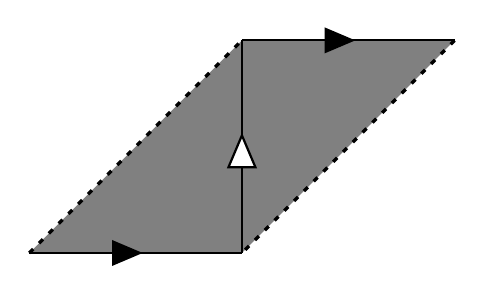
\begin{tikzpicture}[scale=0.9]
    % Grey Filling
    \draw [draw=none, fill=gray] (0, 0) -- (3, 3) -- (6, 3) -- (3, 0);
    % Sides
    \draw [very thick, dash pattern=on 2pt off 3pt] (0, 0) -- (3, 3);
    \draw [thick] (3, 3) -- (6, 3);
    \draw [very thick, dash pattern=on 2pt off 3pt] (6, 3) -- (3, 0);
    \draw [thick] (0, 0) -- (3, 0);
    % Diagonal
    \draw [thick] (3, 0) -- (3, 3);
    % Triangluar black arrows
    \tikzset{arrows={-Triangle[angle=45:12pt, black, fill=black]}};
    \draw [thick] (4.5, 3) -- (4.6, 3);
    \draw [thick] (1.5, 0) -- (1.6, 0);
    % Triangluar white arrow
    \tikzset{arrows={-Triangle[angle=45:14pt, black, fill=white]}};
    \draw [thick] (3, 1.6) -- (3, 1.7);
    \end{tikzpicture}
    \caption*{Parallelogram without left and right sides constructed from the square without diagonal.}
\end{figure}

Then it is easy to see that the space shown above is homeomorphic to the space
$(0, 1) \times S^1$ which is an open annulus (we can continuously deform this parallelogram
to get an open annulus).

\begin{figure}[H]
    \centering
    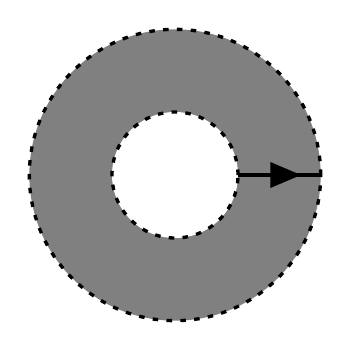
\begin{tikzpicture}
        \draw [very thick, fill=gray, dash pattern=on 2pt off 3pt] (0, 0) circle (1.85cm);
        \draw [very thick, fill=white, dash pattern=on 2pt off 3pt] (0, 0) circle (0.8cm);
        \draw [very thick] (0.8, 0) -- (1.85, 0);
        \tikzset{arrows={-Triangle[angle=45:12pt, black, fill=black]}};
        \draw [thick] (1.4, 0) -- (1.6, 0);
    \end{tikzpicture}
    \caption*{An open annulus.}
\end{figure}

Notice $(0, 1)$ and $S^1$ are both path connected and therefore,
as we have proven in the previous section, the product of two path connected spaces is
connected and $(0, 1) \times S^1$ is path connected. Finally, we conclude that the safe
configuration space $SC^2(S^1)$ is also path connected and therefore, robots $R_1$ and
$R_2$ are freely transportable in the space $S^1$.

%%%%%%%%%%%%%%%%%%%%%%%%%%%%%%%%%%%%%%%%%%%%%%%%%%%%%%%%%%%%%%%%%%%%%%%%%%%%%%%%%%%%%%%%%%%%%%%%%%%%

\subsection*{\centering Motion on $Y$-shaped topological graph}
\addcontentsline{toc}{subsection}{Motion on $Y$-shaped topological graph}
Consider two robots $R_1$ and $R_2$ moving through the $Y$-shaped topological graph.
We, once again, model these AVGs as points moving through this space and denote the space by $Y$.

\begin{figure}[H]
    \centering
    \begin{tikzpicture}[scale=0.5]
        % Branches
        \draw [very thick] (0, 0) -- (-5, 0);
        \draw [very thick] (0, 0) -- (3, 4);
        \draw [very thick] (0, 0) -- (3, -4);
    \end{tikzpicture}
    \caption*{$Y$-shaped topological graph.}
\end{figure}

The safe configuration space for this graph is $SC^2(Y) = Y \times Y - \Delta$ where $\Delta$ is the set
of all points where the coordinate of $R_1$ is the same as that of $R_2$. Thus, $\Delta$ is the set of all
points where we have a collision. With the picture we have now, it is very difficult to determine the free
transportability of the robots in this space. Therefore, we first need to simplify this problem and deal
with smaller sub-problems.

\bigskip

Notice that letter $Y$ is composed by putting three branches together. Let us use this fact and consider
each of these three branches independently. For simplicity, we call these branches $\alpha$, $\beta$, and $\gamma$.

\begin{figure}[H]
    \centering
    \begin{tikzpicture}[scale=0.5]
        % Branches
        \draw [very thick] (0, 0) -- (-5, 0);
        \draw [very thick] (0, 0) -- (3, 4);
        \draw [very thick] (0, 0) -- (3, -4);
        % % Points
        \node [above] at (-3, 0.25) {$\alpha$};
        \node [below] at (2.75, 3) {$\beta$};
        \node [below] at (1.25, -2.5) {$\gamma$};
    \end{tikzpicture}
    \caption*{$Y$-shaped topological graph with branches $\alpha$, $\beta$, and $\gamma$.}
\end{figure}

Then we can rewrite the safe configuration space $SC^2(Y)$ in terms of $\alpha$, $\beta$, and $\gamma$.

$$SC^2(Y) = ((Y \times \alpha) - \Delta)) \cup ((Y \times \beta) - \Delta)) \cup ((Y \times \gamma) - \Delta)).$$

We can now explore each of the subsets of $SC^2$ and then find the way to glue them together to obtain $SC^2(Y)$.

\bigskip

Without a loss of generality, let us consider the configuration space $(Y \times \alpha) - \Delta$.
Notice that $Y$ is already a two-dimensional space. If we multiply it by $\alpha$ we are basically
replicating $Y$ and putting the copies on top of it (think of how one calculates the volume of a cylinder).

\begin{figure}[H]
    \centering
    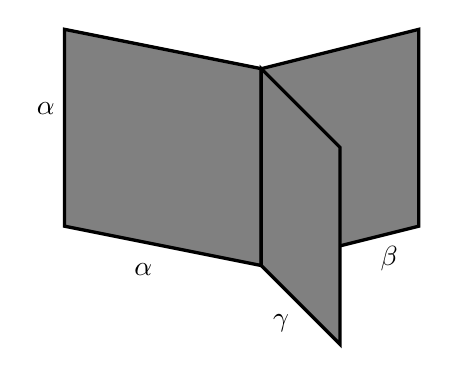
\begin{tikzpicture}[scale=0.5]
        % Branches
        \draw [very thick, fill=gray] (0, 0) -- (-5, 1) -- (-5, 6) -- (0, 5) -- (0, 0);
        \draw [very thick, fill=gray] (0, 0) -- (0, 5) -- (4, 6) -- (4, 1) -- (0, 0);
        \draw [very thick, fill=gray] (0, 0) -- (0, 5) -- (2, 3) -- (2, -2) -- (0, 0);
        % Points
        \node [above] at (-3, -0.5) {$\alpha$};
        \node [below] at (3.25, 0.75) {$\beta$};
        \node [below] at (0.5, -1) {$\gamma$};
        \node [left] at (-5, 4) {$\alpha$};
    \end{tikzpicture}
    \caption*{$C^2(Y \times \alpha)$ configuration space.}
\end{figure}

Now, let us see how the safe configuration space $SC^2(Y \times \alpha)$ would look like.

\begin{figure}[H]
    \centering
    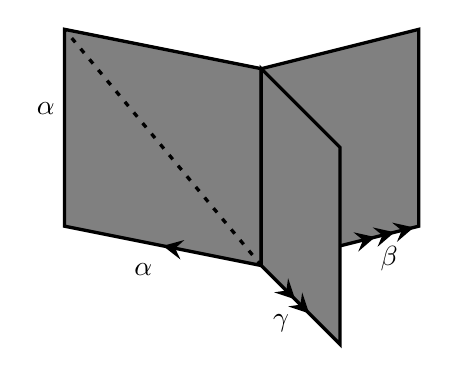
\begin{tikzpicture}[scale=0.5]
        % Branches
        \draw [very thick, fill=gray] (0, 0) -- (-5, 1) -- (-5, 6) -- (0, 5) -- (0, 0);
        \draw [very thick, fill=gray] (0, 0) -- (0, 5) -- (4, 6) -- (4, 1) -- (0, 0);
        \draw [very thick, fill=gray] (0, 0) -- (0, 5) -- (2, 3) -- (2, -2) -- (0, 0);
        % Points
        \node [above] at (-3, -0.5) {$\alpha$};
        \node [below] at (3.25, 0.75) {$\beta$};
        \node [below] at (0.5, -1) {$\gamma$};
        \node [left] at (-5, 4) {$\alpha$};
        % Arrows
        \draw [draw=none, decoration={markings, mark=at position 1 with
            {\arrow[scale=2.25, >=stealth]{>}}}, postaction={decorate}] (0, 0) -- (-2.5, 0.5);
        \draw [draw=none, decoration={markings, mark=at position 1 with
            {\arrow[scale=2.25, >=stealth]{<<}}}, postaction={decorate}] (2, -2) -- (0.5, -0.5);
        \draw [draw=none, decoration={markings, mark=at position 1 with
            {\arrow[scale=2.25, >=stealth]{<<<}}}, postaction={decorate}] (4, 1) -- (2.4, 0.6);
        % Diagonal
        \draw [very thick, dash pattern=on 2pt off 3pt] (0, 0) -- (-5, 6);
    \end{tikzpicture}
    \caption*{$SC^2(Y \times \alpha)$ safe configuration space.}
\end{figure}

The picture above shows the safe configuration space for $C^2(Y \times \alpha)$.
Notice that the square $\alpha \times \alpha$ is the case we already covered when
we had a motion on the line $L$. The diagonal is the set of all points where robot
$R_1$ and $R_2$ have the same coordinates and therefore we exclude it.
Thus, the safe configuration space is really everything of $C^2(Y \times \alpha)$
but the diagonal. The safe configuration space is therefore split into the isosceles
right triangle formed by sides $\alpha$ and $\alpha$, and the rest which is shown on
the picture.

\bigskip

It is easy to see that the rest of the cases are very similar to this.
Here are safe configuration spaces for $C^2(Y \times \beta)$ and $C^2(Y \times \gamma)$.

\begin{figure}[H]
    \centering
    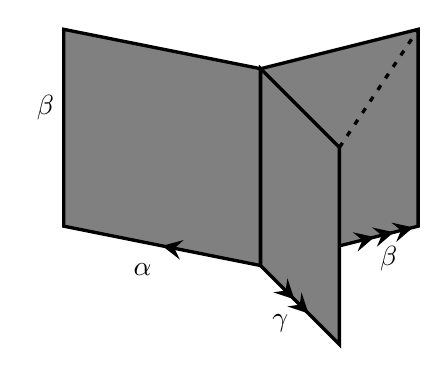
\begin{tikzpicture}[scale=0.5]
        % Branches
        \draw [very thick, fill=gray] (0, 0) -- (-5, 1) -- (-5, 6) -- (0, 5) -- (0, 0);
        \draw [very thick, fill=gray] (0, 0) -- (0, 5) -- (4, 6) -- (4, 1) -- (0, 0);
        \draw [very thick, fill=gray] (0, 0) -- (0, 5) -- (2, 3) -- (2, -2) -- (0, 0);
        % Points
        \node [above] at (-3, -0.5) {$\alpha$};
        \node [below] at (3.25, 0.75) {$\beta$};
        \node [below] at (0.5, -1) {$\gamma$};
        \node [left] at (-5, 4) {$\beta$};
        % Arrows
        \draw [draw=none, decoration={markings, mark=at position 1 with
            {\arrow[scale=2.25, >=stealth]{>}}}, postaction={decorate}] (0, 0) -- (-2.5, 0.5);
        \draw [draw=none, decoration={markings, mark=at position 1 with
            {\arrow[scale=2.25, >=stealth]{<<}}}, postaction={decorate}] (2, -2) -- (0.5, -0.5);
        \draw [draw=none, decoration={markings, mark=at position 1 with
            {\arrow[scale=2.25, >=stealth]{<<<}}}, postaction={decorate}] (4, 1) -- (2.4, 0.6);
        % Diagonal
        \draw [very thick, dash pattern=on 2pt off 3pt] (2, 3) -- (4, 6);
    \end{tikzpicture}
    \qquad
    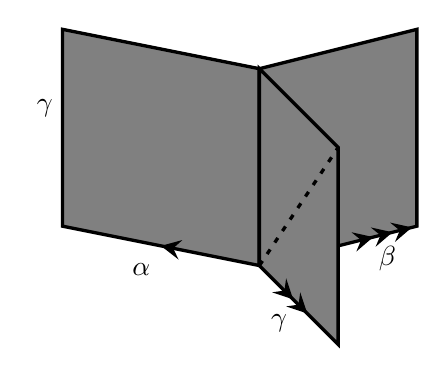
\begin{tikzpicture}[scale=0.5]
        % Branches
        \draw [very thick, fill=gray] (0, 0) -- (-5, 1) -- (-5, 6) -- (0, 5) -- (0, 0);
        \draw [very thick, fill=gray] (0, 0) -- (0, 5) -- (4, 6) -- (4, 1) -- (0, 0);
        \draw [very thick, fill=gray] (0, 0) -- (0, 5) -- (2, 3) -- (2, -2) -- (0, 0);
        % Points
        \node [above] at (-3, -0.5) {$\alpha$};
        \node [below] at (3.25, 0.75) {$\beta$};
        \node [below] at (0.5, -1) {$\gamma$};
        \node [left] at (-5, 4) {$\gamma$};
        % Arrows
        \draw [draw=none, decoration={markings, mark=at position 1 with
            {\arrow[scale=2.25, >=stealth]{>}}}, postaction={decorate}] (0, 0) -- (-2.5, 0.5);
        \draw [draw=none, decoration={markings, mark=at position 1 with
            {\arrow[scale=2.25, >=stealth]{<<}}}, postaction={decorate}] (2, -2) -- (0.5, -0.5);
        \draw [draw=none, decoration={markings, mark=at position 1 with
            {\arrow[scale=2.25, >=stealth]{<<<}}}, postaction={decorate}] (4, 1) -- (2.4, 0.6);
        % Diagonal
        \draw [very thick, dash pattern=on 2pt off 3pt] (0, 0) -- (2, 3);
    \end{tikzpicture}
    \caption*{$SC^2(Y \times \beta)$ (to the left) and $SC^2(Y \times \gamma)$ (to the right) safe configuration spaces.}
\end{figure}

Notice that all three safe configuration spaces have arrows. Now, to get a safe configuration space for $C^2(Y \times Y)$,
we take safe configuration spaces for $C^2(Y \times \alpha)$, $C^2(Y \times \beta)$, and $C^2(Y \times \gamma)$ and glue them
together in the way that the arrows match (singles arrows match single arrows, double arrows match double arrows, and triple
arrows match triple arrows). The picture below represents a safe configuration space $SC^2(Y \times Y)$ after the gluing is complete.

\begin{figure}[H]
    \centering
    \begin{turn}{1}
    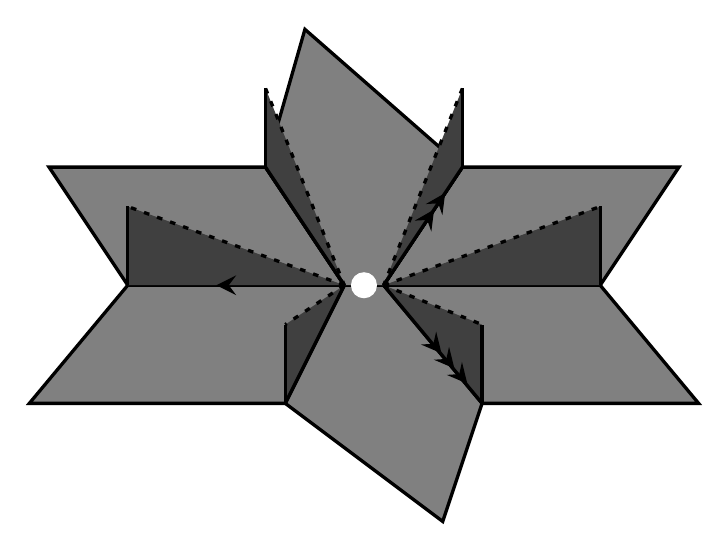
\begin{tikzpicture}[scale=0.5]
        % Petals
        \draw [very thick, fill=gray] (0.5, 0) -- (6, 0) -- (8.5, -3) -- (3, -3) -- (0.5, 0);
        \draw [very thick, fill=gray] (-0.5, 0) -- (-6, 0) -- (-8.5, -3) -- (-2, -3) -- (-0.5, 0);
        \draw [very thick, fill=gray] (-0.5, 0) -- (-2, -3) -- (2, -6) -- (3, -3) -- (0.5, 0) -- (-0.5, 0);
        \draw [very thick, fill=gray] (-6, 0) -- (-8, 3) -- (-2.5, 3) -- (-0.5, 0) -- (-6, 0);
        \draw [very thick, fill=gray] (6, 0) -- (8, 3) -- (2.5, 3) -- (0.5, 0) -- (6, 0);
        \draw [very thick, fill=gray] (-0.5, 0) -- (-2.5, 3) -- (-1.5, 6.5) -- (2.5, 3) -- (0.5, 0) -- (0.5, 0);
        % Triangles
        % 1
        \draw [draw=none, very thick, fill=darkgray] (0.5, 0) -- (6, 0) -- (6, 2) -- (0.5, 0);
        \draw [very thick, dash pattern=on 2pt off 3pt] (0.5, 0) -- (6, 2);
        \draw [very thick] (6, 0) -- (6, 2);
        \draw [very thick] (6, 2) -- (6, 0);
        % 2
        \draw [draw=none, very thick, fill=darkgray] (-0.5, 0) -- (-6, 0) -- (-6, 2) -- (-0.5, 0);
        \draw [very thick, dash pattern=on 2pt off 3pt] (-0.5, 0) -- (-6, 2);
        \draw [very thick] (-6, 0) -- (-6, 2);
        \draw [very thick] (-6, 2) -- (-6, 0);
        % 3
        \draw [draw=none, very thick, fill=darkgray] (0.5, 0) -- (3, -3) -- (3, -1) -- (0.5, 0);
        \draw [very thick, dash pattern=on 2pt off 3pt] (0.5, 0) -- (3, -1);
        \draw [very thick] (3, -3) -- (3, -1);
        \draw [very thick] (3, -3) -- (0.5, 0);
        % 4
        \draw [draw=none, very thick, fill=darkgray] (-0.5, 0) -- (-2, -3) -- (-2, -1) -- (-0.5, 0);
        \draw [very thick, dash pattern=on 2pt off 3pt] (-0.5, 0) -- (-2, -1);
        \draw [very thick] (-0.5, 0) -- (-2, -3);
        \draw [very thick] (-2, -3) -- (-2, -1);
        % 5
        \draw [draw=none, very thick, fill=darkgray] (-0.5, 0) -- (-2.5, 3) -- (-2.5, 5) -- (-0.5, 0);
        \draw [very thick, dash pattern=on 2pt off 3pt] (-2.5, 5) -- (-0.5, 0);
        \draw [very thick] (-2.5, 3) -- (-2.5, 5);
        \draw [very thick] (-0.5, 0) -- (-2.5, 3);
        % 6
        \draw [draw=none, very thick, fill=darkgray] (0.5, 0) -- (2.5, 3) -- (2.5, 5) -- (0.5, 0);
        \draw [very thick, dash pattern=on 2pt off 3pt] (2.5, 5) -- (0.5, 0);
        \draw [very thick] (2.5, 3) -- (0.5, 0);
        \draw [very thick] (2.5, 5) -- (2.5, 3);
        % The dot
        \draw [white, fill=white] (0, 0) circle (9pt);
        % Arrows
        \draw [draw=none, decoration={markings, mark=at position 1 with
            {\arrow[scale=2.25, >=stealth]{>}}}, postaction={decorate}] (-0.5, 0) -- (-3.75, 0);
        \draw [draw=none, decoration={markings, mark=at position 1 with
            {\arrow[scale=2.25, >=stealth]{<<}}}, postaction={decorate}] (2.5, 3) -- (1.5, 1.5);
        \draw [draw=none, decoration={markings, mark=at position 1 with
            {\arrow[scale=2.25, >=stealth]{>>>}}}, postaction={decorate}] (0.5, 0) -- (2.625, -2.5);
    \end{tikzpicture}
    \end{turn}
    \caption*{$SC^2(Y \times Y)$ safe configuration space.}
\end{figure}

The empty hole in the middle corresponds to both robots being in the intersection of $\alpha$, $\beta$, and $\gamma$.
Now, notice that this configuration space is path connected since every pair of points in $SC^2(Y \times Y)$ can be joined
by a path in $SC^2(Y \times Y)$. Therefore, every configuration is attainable from every other one and thus, AVGs
$R_1$ and $R_2$ are freely transportable in $Y$.

%%%%%%%%%%%%%%%%%%%%%%%%%%%%%%%%%%%%%%%%%%%%%%%%%%%%%%%%%%%%%%%%%%%%%%%%%%%%%%%%%%%%%%%%%%%%%%%%%%%%

\begin{center}
\begin{thebibliography}{00}
    \bibitem{1} Adams C. and Fransoza R., ``Introduction to Topology'', 2008, p. 105.
    \bibitem{2} Adams C. and Fransoza R., ``Introduction to Topology'', 2008, pp. 105 -- 106.
    \bibitem{3} Munkres J. R., ``Topology'', 2000, Second Edition, Upper Saddle River, NJ: Prentice Hall., p. 76.
    \bibitem{4} Munkres J. R., ``Topology'', 2000, Second Edition, Upper Saddle River, NJ: Prentice Hall., p. 76.
    \bibitem{5} Thomas G. B., ``Thomas' Calculus", 2010, Thirteenth Edition, p. 77.
    \bibitem{6} Munkres J. R., ``Topology'', 2000, Second Edition, Upper Saddle River, NJ: Prentice Hall., p. 102.
    \bibitem{7} Munkres J. R., ``Topology'', 2000, Second Edition, Upper Saddle River, NJ: Prentice Hall., p. 105.
    \bibitem{8} Munkres J. R., ``Topology'', 2000, Second Edition, Upper Saddle River, NJ: Prentice Hall., p. 148.
    \bibitem{9} Munkres J. R., ``Topology'', 2000, Second Edition, Upper Saddle River, NJ: Prentice Hall., p. 155.
    \bibitem{10} Basener W. F., ``Topology and Its Applications'', 2006, p. 65.
    \bibitem{11} Munkres J. R., ``Topology'', 2000, Second Edition, Upper Saddle River, NJ: Prentice Hall., p. 108.
    \bibitem{12} Lynch K. and Park F., ``Modern Robotics: Mechanics, Planning, and Control'', Chapter 2.1, \href{https://youtube.com/watch?v=z29hYlagOYM}{https://youtube.com/watch?v=z29hYlagOYM}.
    \bibitem{13} Adams C. and Fransoza R., ``Introduction to Topology'', 2008, p. 199.
    \bibitem{14} Adams C. and Fransoza R., ``Introduction to Topology'', 2008, p. 199.
    \bibitem{15} Mackevicius E., ``Configuration Spaces'', 2008, p. 9,\\\href{https://math.uchicago.edu/~may/VIGRE/VIGRE2009/REUPapers/Mackevicius.pdf}{https://math.uchicago.edu/~may/VIGRE/VIGRE2009/REUPapers/Mackevicius.pdf}.
\end{thebibliography}
\addcontentsline{toc}{section}{References}
\end{center}

\end{document}
